\documentclass[aspectratio=169,handout]{beamer}
\usepackage[utf8]{inputenc}
\usepackage{color}
\usepackage{tikz}
\usepackage{gensymb}
\usepackage{multirow}
\usepackage{algorithm}
\usepackage{algorithmic}
\usetikzlibrary{shapes,shapes.multipart}

\definecolor{color}{RGB}{68,197,193}

\usetheme{Berlin}

\usecolortheme[named=color]{structure}
\useoutertheme{split}
\useinnertheme{rectangles}

\setbeamertemplate{caption}[numbered]

\title[IIC3633]{Using Collective Matrix Factorization and Tags to improve a Recommender System}
\author{Cristopher Arenas}
\institute{PUC, Campus San Joaquín}
%\date{Wednesday, November 25th of 2015}

\begin{document}

\begin{frame}
\maketitle
\end{frame}

\begin{frame}
\frametitle{Introduction}
\begin{itemize}
\item Recommender Systems are used to provide recommendation to users about items
\item The problem consist in predict for an user $u$ the preference about an item $i$, tipically with a range of values $r$.
\end{itemize}
\end{frame}

\begin{frame}
\frametitle{Introduction}
\begin{itemize}
\item There are methods based in Collaborative Filter to resolve the problem.
\item This approach find similarities
\begin{itemize}
\item Users
\item Items
\item Ratings
\end{itemize}
\end{itemize}
\end{frame}

\begin{frame}
\frametitle{Introduction}
\begin{itemize}
\item One of the major problems with CF is the \textbf{sparsity problem}.
\item The most of users rating a few items.
\pause
\item Some Matrix Factorization methods are used to solve the sparsity problem using filling techniques.
\end{itemize}
\end{frame}

\begin{frame}
\frametitle{Introduction}
\begin{itemize}
\item A method called Collective Matrix Factorization will be proposed.
\pause
\item The use of tag information will be considered.
\end{itemize}
\end{frame}

\begin{frame}
\frametitle{Related Work}
\begin{itemize}
\item Matrix Factorization Techniques consider the factorization of a matrix that relates users and items.
\pause
\item Traditional approaches try to minimize the error function:
\begin{equation}
E = \sum_{(u,i)\in K} (r_{ui}-q_i^Tp_{u})^2 + \lambda(||q_i||^2+||p_u||^2)
\end{equation}
\end{itemize}
\end{frame}

\begin{frame}
\frametitle{Proposed Method}
There are three matrices that relates $m$ users, $n$ items and $p$ tags: \pause
\begin{itemize}
\item $U(u,i)$: user-item matrix. Shows the \textit{rating} of user $u$ for an item $i$.\pause
\item $T(u,t)$: user-tag matrix. Shows the \textit{preference} of an user $u$ for the tag $t$.\pause
\item $G(i,t)$: tag-item matrix. Shows \textit{relevance} between item $i$ and tag $t$.
\end{itemize}
\end{frame}

\begin{frame}
\frametitle{Proposed Method}
\begin{itemize}
\item $U(u,i)$ and $G(i,t)$ are constructed directly with information.
\pause
\item $T$ is constructed using $U$ and $G$.
\end{itemize}
\begin{equation}
\label{eq:t}
T(u,t) = \frac{1}{N} \sum_{k=1}^{n}U(u,k) \times G(k,t)
\end{equation}
\end{frame}

\begin{frame}
\frametitle{Proposed Method}
\begin{itemize}
\item Later, submatrices $X$, $Y$ and $Z$ are used to construct two matrices $U'$ and $T'$.
\end{itemize}
\begin{equation}
\label{eq:u}
U' = XY^T
\end{equation} 

\begin{equation}
\label{eq:u}
T' = XZ^T
\end{equation} 
\end{frame}

\begin{frame}
\frametitle{Proposed Method}
\begin{itemize}
\item Gradient Descent Method (GDM) is performed to minimize the error between real values and approximated values:
\begin{equation}
\label{eq:error}
\begin{aligned}
ER(X,Y,Z) &= \frac{1}{2}||J \circ (U-XY^T)||^{2}_{F}+\frac{\alpha}{2}||T-XZ^T||^{2}_{F}\\
&+\frac{\beta}{2}\left( ||X||^{2}_{F} + ||Y||^{2}_{F} + ||Z||^{2}_{F} \right)
\end{aligned}
\end{equation}
\pause
\item Gradients are calculated:
\begin{equation}
\label{eq:gradientx}
\nabla_XER = \left[ J \circ (XY^T-U) \right] Y + \alpha (XZ^T-T)Z + \beta X
\end{equation}
\begin{equation}
\label{eq:gradienty}
\nabla_YER = \left[ J \circ (XY^T-U) \right] X + \beta Y
\end{equation}
\begin{equation}
\label{eq:gradientz}
\nabla_ZER = \alpha (XZ^T-T)X + \beta Z
\end{equation}
\end{itemize}
\end{frame}

\begin{frame}
\frametitle{Proposed Method}
\begin{algorithm}[H]
\caption{Gradient Descent Method}
\label{alg:gdm}
\begin{algorithmic}[1]
\STATE Initialize $X$, $Y$, $Z$ with random number in range (0,1)
\STATE $t = 0$
\WHILE{$t < max\_iteration$}
\STATE Get gradients $\nabla_XER$, $\nabla_YER$ and $\nabla_ZER$.
\STATE $\gamma=1$
\WHILE{$(ER(X_t-\gamma\nabla_{X_t},Y_t-\gamma\nabla_{Y_t},Z_t-\gamma\nabla_{Z_t})>ER(X_t,Y_t,Z_t))$}
\STATE $\gamma = \gamma/2$
\ENDWHILE
\STATE $X_{t+1} = X_{t}-\gamma\nabla_{X_t}$
\STATE $Y_{t+1} = Y_{t}-\gamma\nabla_{Y_t}$
\STATE $Z_{t+1} = Z_{t}-\gamma\nabla_{Z_t}$
\STATE $t = t+1$
\ENDWHILE
\end{algorithmic}
\end{algorithm}
\end{frame}

\begin{frame}
\frametitle{Experiments}
\begin{itemize}
\item Dataset: MovieLens
\begin{itemize}
\item 1.000.209 ratings
\item 3.682 movies
\item 6.040 users
\end{itemize}
\pause
\item Tag-Genome
\begin{itemize}
\item 9.734 movies
\item 1.128 tags
\end{itemize}
\pause
\item 3.642 movies in MovieLens and Tag-Genome
\pause
\item 80\% training and 20\% testing
\end{itemize}
\end{frame}

\begin{frame}
\frametitle{Experiments}
\begin{itemize}
\item 3 experiments:
\pause
\begin{enumerate}
\item Latent factors
\item Prediction: MAE, RMSE
\item Top-N: nDCG
\end{enumerate}
\end{itemize}
\end{frame}

\begin{frame}
\frametitle{Results}
\begin{figure}[!htb]
\centering
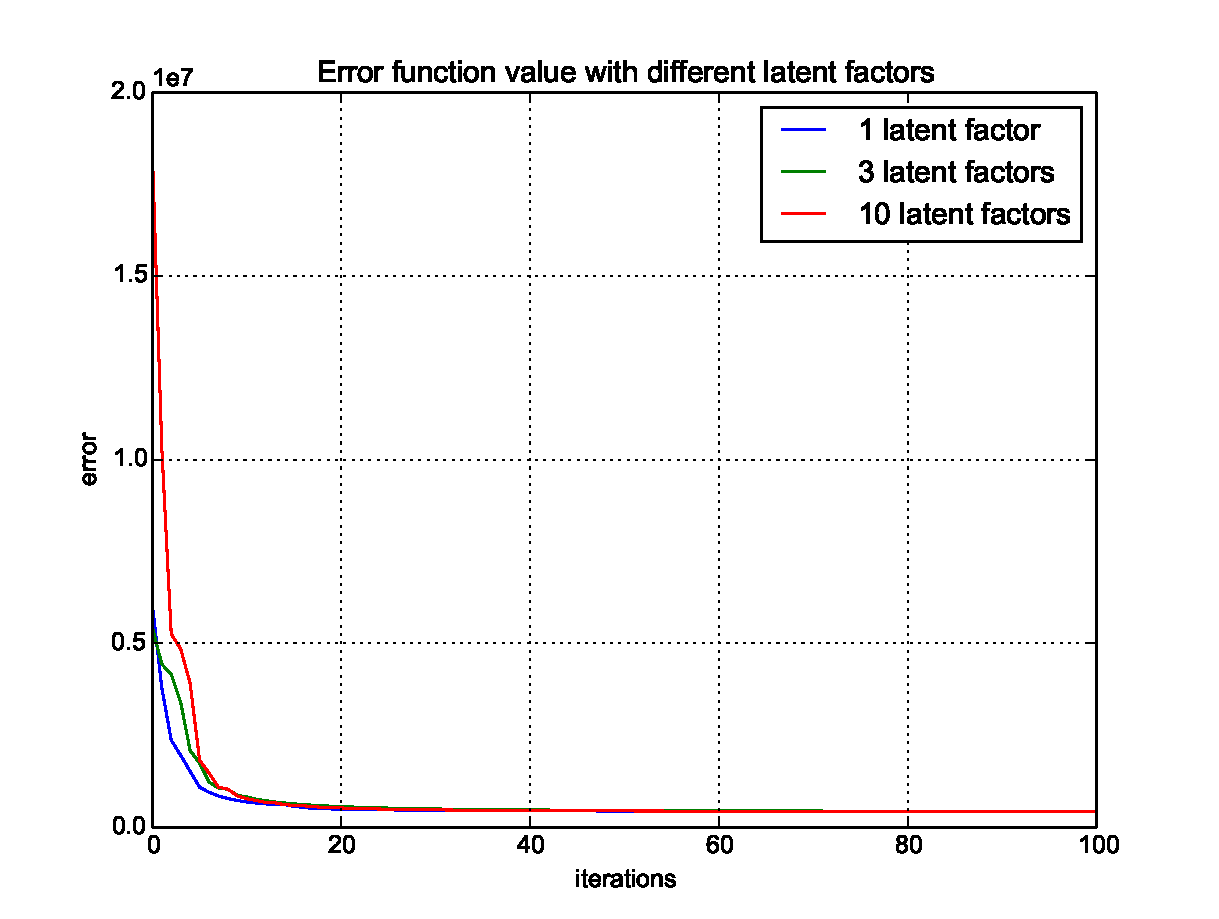
\includegraphics[width=0.6\textwidth]{exp1}
\caption{Error function using three different latent factors.}
\label{fig:error}
\end{figure}
\end{frame}

\begin{frame}
\frametitle{Results}
\begin{table}[!htb]
\caption{MAE and RMSE considering two scenarios.}
\centering
\begin{tabular}{|c|c|c|}
\hline
Metric & With tags & Without tags\\ \hline \hline
$MAE$ & 0.7236 & 0.6961\\ \hline
$RMSE$ & 0.9264 & 0.8945\\
\hline
\end{tabular}
\label{tab:metric1}
\end{table}
\end{frame}

\begin{frame}
\frametitle{Results}
\begin{table}
\centering
\caption{nDCG@p metric for two scenarios and differents values of p}
\begin{tabular}{|c|c|c|c|c|c|c|}
\hline
\multirow{2}{*}{$p$} & \multicolumn{2}{|c|}{Best user} & \multicolumn{2}{|c|}{Worst user} & \multicolumn{2}{|c|}{Average} \\ \cline{2-7}
 & With tags & Without tags & With tags & Without tags & With tags & Without tags \\ \hline \hline
1 & 0.7869 & 0.8354 & 0.7869 & 0.8354 & 0.7869 & 0.8354 \\ \hline
3 & 0.7855 & 0.8323 & 0.6431 & 0.6581 & 0.7169 & 0.7337\\ \hline
5 & 0.7811 & 0.8256 & 0.4256 & 0.5164 & 0.6353 & 0.6740\\ \hline
10 & 0.9966 & 0.8666 & 0.4147 & 0.5002 & 0.6888 & 0.7157\\ \hline
20 & 0.9676 & 0.9658 & 0.3974 & 0.4682 & 0.6798 & 0.7066\\ \hline
\end{tabular}
\label{tab:ndcg}
\end{table}
\end{frame}

\begin{frame}
\frametitle{Conclusions}
\begin{itemize}
\item Different ways to do matrix factorizations.
\pause
\item Purpouse of this work: \pause using tags in a collective matrix factorization.
\pause
\item Latent factors
\pause
\item About results.
\pause
\item Future work: exaustive revision.
\end{itemize}
\end{frame}

\end{document}
